\documentclass[a4paper,12pt]{article} % This defines the style of your paper

\usepackage[top = 2.5cm, bottom = 2.5cm, left = 2.5cm, right = 2.5cm]{geometry} 

% Unfortunately, LaTeX has a hard time interpreting German Umlaute. The following two lines and packages should help. If it doesn't work for you please let me know.
\usepackage[T1]{fontenc}
\usepackage[utf8]{inputenc}
\usepackage{pifont}
% \usepackage{ctex}
\usepackage{amsthm, amsmath, amssymb, mathrsfs,mathtools}
% ---------------------------------------------------------------------
% Program: listings-stata.tex
% Author:  github.com/mcaceresb
% Purpose: Stata language definition for LaTeX listings package
% Usage:   Add \input{listings-stata.tex} to your preamble

% Syntax from
% - https://github.com/isagalaev/highlight.js/blob/master/src/languages/stata.js
% - https://github.com/jpitblado/vim-stata/blob/master/syntax/stata.vim
% - http://fmwww.bc.edu/RePEc/bocode/s/synlightlist.ado

\RequirePackage{listings}
\RequirePackage{color}
\RequirePackage[svgnames]{xcolor}
\definecolor{spRed}{HTML}{BE646C}

% ---------------------------------------------------------------------
% Stata language definition

\lstdefinelanguage{stata}{
  sensitive=true,
  %
  % Macros, global and local
  alsoletter={\{\}0123456789},
  keywordsprefix=\$,
  morecomment=[n][keywordstyle9]{`}{'},
  morekeywords={},
  %
  % Comments
  morecomment=[f][\color{Green}\slshape][0]*,
  morecomment=[l]{//},
  morecomment=[s]{/*}{*/},
  %
  % Strings
  morecomment=[n][\color{Maroon}]{`"}{"'},
  morestring=[b]",
  %
  % Add-ons and system Commands
  morekeywords=[2]{
    if ,else ,in ,foreach ,for ,forv ,forva ,forval ,forvalu ,forvalue
    ,forvalues ,by ,bys ,bysort ,xi ,quietly ,qui ,capture ,about
    ,ac ,ac_7 ,acprplot ,acprplot_7 adjust ,ado ,adopath ,adoupdate
    ,alpha ,ameans ,an ,ano ,anov ,anova ,anova_estat ,anova_terms
    ,anovadef ,aorder ,ap ,app ,appe ,appen ,append ,arch ,arch_dr
    ,arch_estat ,arch_p ,archlm ,areg ,areg_p ,args ,arima ,arima_dr
    ,arima_estat ,arima_p ,as ,asmprobit ,asmprobit_estat ,asmprobit_lf
    ,asmprobit_mfx__dlg ,asmprobit_p ,ass ,asse ,asser ,assert ,avplot
    ,avplot_7 ,avplots ,avplots_7 bcskew0 ,bgodfrey ,binreg ,bip0_lf
    ,biplot ,bipp_lf ,bipr_lf ,bipr_p ,biprobit ,bitest ,bitesti
    ,bitowt ,blogit ,bmemsize ,boot ,bootsamp ,bootstrap ,bootstrap_8
    ,boxco_l ,boxco_p ,boxcox ,boxcox_6 ,boxcox_p ,bprobit ,br ,break
    ,brier ,bro ,brow ,brows ,browse ,brr ,brrstat ,bs ,bs_7 ,bsampl_w
    ,bsample ,bsample_7 ,bsqreg ,bstat ,bstat_7 ,bstat_8 ,bstrap
    ,bstrap_7 ,ca ,ca_estat ,ca_p ,cabiplot ,camat ,canon ,canon_8
    ,canon_8_p ,canon_estat ,canon_p ,cap ,caprojection ,capt ,captu
    ,captur ,capture ,cat ,cc ,cchart ,cchart_7 ,cci ,cd ,censobs_table
    ,centile ,cf ,char ,chdir ,checkdlgfiles ,checkestimationsample
    ,checkhlpfiles ,checksum ,chelp ,ci ,cii ,cl ,class ,classutil
    ,clear ,cli ,clis ,clist ,clo ,clog ,clog_lf ,clog_p ,clogi
    ,clogi_sw ,clogit ,clogit_lf ,clogit_p ,clogitp ,clogl_sw ,cloglog
    ,clonevar ,clslistarray ,cluster ,cluster_measures ,cluster_stop
    ,cluster_tree ,cluster_tree_8 ,clustermat ,cmdlog ,cnr ,cnre
    ,cnreg ,cnreg_p ,cnreg_sw ,cnsreg ,codebook ,collaps4 ,collapse
    ,colormult_nb ,colormult_nw ,compare ,compress ,conf ,confi
    ,confir ,confirm ,conren ,cons ,const ,constr ,constra ,constrai
    ,constrain ,constraint ,continue ,contract ,copy ,copyright
    ,copysource ,cor ,corc ,corr ,corr2data ,corr_anti ,corr_kmo
    ,corr_smc ,corre ,correl ,correla ,correlat ,correlate ,corrgram
    ,cou ,coun ,count ,cox ,cox_p ,cox_sw ,coxbase ,coxhaz ,coxvar
    ,cprplot ,cprplot_7 ,crc ,cret ,cretu ,cretur ,creturn ,cross ,cs
    ,cscript ,cscript_log ,csi ,ct ,ct_is ,ctset ,ctst_5 ,ctst_st
    ,cttost ,cumsp ,cumsp_7 ,cumul ,cusum ,cusum_7 ,cutil ,d ,datasig
    ,datasign ,datasigna ,datasignat ,datasignatu ,datasignatur
    ,datasignature ,datetof ,db ,dbeta ,de ,dec ,deco ,decod ,decode
    ,deff ,des ,desc ,descr ,descri ,describ ,describe ,destring
    ,dfbeta ,dfgls ,dfuller ,di ,di_g ,dir ,dirstats ,dis ,discard
    ,disp ,disp_res ,disp_s ,displ ,displa ,display ,distinct ,do
    ,doe ,doed ,doedi ,doedit ,dotplot ,dotplot_7 ,dprobit ,drawnorm
    ,drop ,ds ,ds_util ,dstdize ,duplicates ,durbina ,dwstat ,dydx ,e
    ,ed ,edi ,edit ,egen ,eivreg ,emdef ,en ,enc ,enco ,encod ,encode
    ,eq ,erase ,ereg ,ereg_lf ,ereg_p ,ereg_sw ,ereghet ,ereghet_glf
    ,ereghet_glf_sh ,ereghet_gp ,ereghet_ilf ,ereghet_ilf_sh ,ereghet_ip
    ,eret ,eretu ,eretur ,ereturn ,err ,erro ,error ,est ,est_cfexist
    ,est_cfname ,est_clickable ,est_expand ,est_hold ,est_table
    ,est_unhold ,est_unholdok ,estat ,estat_default ,estat_summ
    ,estat_vce_only ,esti ,estimates ,etodow ,etof ,etomdy ,ex ,exi
    ,exit ,expand ,expandcl ,fac ,fact ,facto ,factor ,factor_estat
    ,factor_p ,factor_pca_rotated ,factor_rotate ,factormat ,fcast
    ,fcast_compute ,fcast_graph ,fdades ,fdadesc ,fdadescr ,fdadescri
    ,fdadescrib ,fdadescribe ,fdasav ,fdasave ,fdause ,fh_st ,file
    ,open ,file ,read ,file ,close ,file ,filefilter ,fillin
    ,find_hlp_file ,findfile ,findit ,findit_7 ,fit ,fl ,fli ,flis
    ,flist ,for5_0 ,form ,forma ,format ,fpredict ,frac_154 ,frac_adj
    ,frac_chk ,frac_cox ,frac_ddp ,frac_dis ,frac_dv ,frac_in ,frac_mun
    ,frac_pp ,frac_pq ,frac_pv ,frac_wgt ,frac_xo ,fracgen ,fracplot
    ,fracplot_7 ,fracpoly ,fracpred ,fron_ex ,fron_hn ,fron_p ,fron_tn
    ,fron_tn2 ,frontier ,ftodate ,ftoe ,ftomdy ,ftowdate ,g ,gamhet_glf
    ,gamhet_gp ,gamhet_ilf ,gamhet_ip ,gamma ,gamma_d2 ,gamma_p
    ,gamma_sw ,gammahet ,gdi_hexagon ,gdi_spokes ,ge ,gen ,gene ,gener
    ,genera ,generat ,generate ,genrank ,genstd ,genvmean ,gettoken
    ,gl ,gladder ,gladder_7 ,glim_l01 ,glim_l02 glim_l03 ,glim_l04
    ,glim_l05 ,glim_l06 ,glim_l07 ,glim_l08 ,glim_l09 ,glim_l10 glim_l11
    ,glim_l12 ,glim_lf ,glim_mu ,glim_nw1 ,glim_nw2 ,glim_nw3 ,glim_p
    ,glim_v1 ,glim_v2 ,glim_v3 ,glim_v4 ,glim_v5 ,glim_v6 ,glim_v7 ,glm
    ,glm_6 glm_p ,glm_sw ,glmpred ,glo ,glob ,globa ,global ,glogit
    ,glogit_8 ,glogit_p ,gmeans ,gnbre_lf ,gnbreg ,gnbreg_5 ,gnbreg_p
    ,gomp_lf ,gompe_sw ,gomper_p ,gompertz ,gompertzhet ,gomphet_glf
    ,gomphet_glf_sh ,gomphet_gp ,gomphet_ilf ,gomphet_ilf_sh ,gomphet_ip
    ,gphdot ,gphpen ,gphprint ,gprefs ,gprobi_p ,gprobit ,gprobit_8
    ,gr ,gr7 ,gr_copy ,gr_current ,gr_db ,gr_describe ,gr_dir ,gr_draw
    ,gr_draw_replay ,gr_drop ,gr_edit ,gr_editviewopts ,gr_example
    ,gr_example2 gr_export ,gr_print ,gr_qscheme ,gr_query ,gr_read
    ,gr_rename ,gr_replay ,gr_save ,gr_set ,gr_setscheme ,gr_table
    ,gr_undo ,gr_use ,graph ,graph7 grebar ,greigen ,greigen_7
    ,greigen_8 ,grmeanby ,grmeanby_7 ,gs_fileinfo ,gs_filetype
    ,gs_graphinfo ,gs_stat ,gsort ,gwood ,h ,hadimvo ,hareg ,hausman
    ,haver ,he ,heck_d2 ,heckma_p ,heckman ,heckp_lf ,heckpr_p ,heckprob
    ,hel ,help ,hereg ,hetpr_lf ,hetpr_p ,hetprob ,hettest ,hexdump
    ,hilite ,hist ,hist_7 histogram ,hlogit ,hlu ,hmeans ,hotel
    ,hotelling ,hprobit ,hreg ,hsearch ,icd9 ,icd9_ff ,icd9p ,iis
    ,impute ,imtest ,inbase ,include ,inf ,infi ,infil ,infile ,infix
    ,inp ,inpu ,input ,ins ,insheet ,insp ,inspe ,inspec ,inspect ,integ
    ,inten ,intreg ,intreg_7 ,intreg_p ,intrg2_ll ,intrg_ll ,intrg_ll2
    ,ipolate ,iqreg ,ir ,irf ,irf_create ,irfm ,iri ,is_svy ,is_svysum
    ,isid ,istdize ,ivprob_1_lf ,ivprob_lf ,ivprobit ,ivprobit_p ,ivreg
    ,ivreg_footnote ,ivtob_1_lf ,ivtob_lf ,ivtobit ,ivtobit_p ,jackknife
    ,jacknife ,jknife ,jknife_6 ,jknife_8 ,jkstat ,joinby ,kalarma1
    ,kap ,kap_3 ,kapmeier ,kappa ,kapwgt ,kdensity ,kdensity_7 keep
    ,ksm ,ksmirnov ,ktau ,kwallis ,l ,la ,lab ,labe ,label ,labelbook
    ,ladder ,levels ,levelsof ,leverage ,lfit ,lfit_p ,li ,lincom ,line
    ,linktest ,lis ,list ,lloghet_glf ,lloghet_glf_sh ,lloghet_gp
    ,lloghet_ilf ,lloghet_ilf_sh ,lloghet_ip ,llogi_sw ,llogis_p
    ,llogist ,llogistic ,llogistichet ,lnorm_lf ,lnorm_sw ,lnorma_p
    ,lnormal ,lnormalhet ,lnormhet_glf ,lnormhet_glf_sh ,lnormhet_gp
    ,lnormhet_ilf ,lnormhet_ilf_sh ,lnormhet_ip ,lnskew0 ,loadingplot
    ,loc ,loca ,local ,log ,logi ,logis_lf ,logistic ,logistic_p
    ,logit ,logit_estat ,logit_p ,loglogs ,logrank ,loneway ,lookfor
    ,lookup ,lowess ,lowess_7 ,lpredict ,lrecomp ,lroc ,lroc_7 ,lrtest
    ,ls ,lsens ,lsens_7 ,lsens_x ,lstat ,ltable ,ltable_7 ,ltriang
    ,lv ,lvr2plot ,lvr2plot_7 ,m ,ma ,mac ,macr ,macro ,makecns ,man
    ,manova ,manova_estat ,manova_p ,manovatest ,mantel ,mark ,markin
    ,markout ,marksample ,mat ,mat_capp ,mat_order ,mat_put_rr ,mat_rapp
    ,mata ,mata_clear ,mata_describe ,mata_drop ,mata_matdescribe
    ,mata_matsave ,mata_matuse ,mata_memory ,mata_mlib ,mata_mosave
    ,mata_rename ,mata_which ,matalabel ,matcproc ,matlist ,matname
    ,matr ,matri ,matrix ,matrix_input__dlg ,matstrik ,mcc ,mcci ,md0_
    ,md1_ ,md1debug_ ,md2_ ,md2debug_ ,mds ,mds_estat ,mds_p ,mdsconfig
    ,mdslong ,mdsmat ,mdsshepard ,mdytoe ,mdytof ,me_derd ,mean ,means
    ,median ,memory ,memsize ,meqparse ,mer ,merg ,merge ,mfp ,mfx
    ,mhelp ,mhodds ,minbound ,mixed_ll ,mixed_ll_reparm ,mkassert
    ,mkdir ,mkmat ,mkspline ,ml ,ml_5 ml_adjs ,ml_bhhhs ,ml_c_d
    ,ml_check ,ml_clear ,ml_cnt ,ml_debug ,ml_defd ,ml_e0 ml_e0_bfgs
    ,ml_e0_cycle ,ml_e0_dfp ,ml_e0i ,ml_e1 ,ml_e1_bfgs ,ml_e1_bhhh
    ,ml_e1_cycle ,ml_e1_dfp ,ml_e2 ,ml_e2_cycle ,ml_ebfg0 ,ml_ebfr0
    ,ml_ebfr1 ml_ebh0q ,ml_ebhh0 ,ml_ebhr0 ,ml_ebr0i ,ml_ecr0i ,ml_edfp0
    ,ml_edfr0 ,ml_edfr1 ml_edr0i ,ml_eds ,ml_eer0i ,ml_egr0i ,ml_elf
    ,ml_elf_bfgs ,ml_elf_bhhh ,ml_elf_cycle ,ml_elf_dfp ,ml_elfi
    ,ml_elfs ,ml_enr0i ,ml_enrr0 ,ml_erdu0 ml_erdu0_bfgs ,ml_erdu0_bhhh
    ,ml_erdu0_bhhhq ,ml_erdu0_cycle ,ml_erdu0_dfp ,ml_erdu0_nrbfgs
    ,ml_exde ,ml_footnote ,ml_geqnr ,ml_grad0 ,ml_graph ,ml_hbhhh
    ,ml_hd0 ,ml_hold ,ml_init ,ml_inv ,ml_log ,ml_max ,ml_mlout
    ,ml_mlout_8 ,ml_model ,ml_nb0 ,ml_opt ,ml_p ,ml_plot ,ml_query
    ,ml_rdgrd ,ml_repor ,ml_s_e ,ml_score ,ml_searc ,ml_technique
    ,ml_unhold ,mleval ,mlf_ ,mlmatbysum ,mlmatsum ,mlog ,mlogi ,mlogit
    ,mlogit_footnote ,mlogit_p ,mlopts ,mlsum ,mlvecsum ,mnl0_ ,mor
    ,more ,mov ,move ,mprobit ,mprobit_lf ,mprobit_p ,mrdu0_ ,mrdu1_
    ,mvdecode ,mvencode ,mvreg ,mvreg_estat ,n ,nbreg ,nbreg_al
    ,nbreg_lf ,nbreg_p ,nbreg_sw ,nestreg ,net ,newey ,newey_7 ,newey_p
    ,news ,nl ,nl_7 ,nl_9 ,nl_9_p ,nl_p ,nl_p_7 nlcom ,nlcom_p ,nlexp2
    ,nlexp2_7 ,nlexp2a ,nlexp2a_7 ,nlexp3 ,nlexp3_7 ,nlgom3 nlgom3_7
    ,nlgom4 ,nlgom4_7 ,nlinit ,nllog3 ,nllog3_7 ,nllog4 ,nllog4_7
    ,nlog_rd ,nlogit ,nlogit_p ,nlogitgen ,nlogittree ,nlpred ,no
    ,nobreak ,noi ,nois ,noisi ,noisil ,noisily ,note ,notes ,notes_dlg
    ,nptrend ,numlabel ,numlist ,odbc ,old_ver ,olo ,olog ,ologi
    ,ologi_sw ,ologit ,ologit_p ,ologitp ,on ,one ,onew ,onewa ,oneway
    ,op_colnm ,op_comp ,op_diff ,op_inv ,op_str ,opr ,opro ,oprob
    ,oprob_sw ,oprobi ,oprobi_p ,oprobit ,oprobitp ,opts_exclusive
    ,order ,orthog ,orthpoly ,ou ,out ,outf ,outfi ,outfil ,outfile
    ,outs ,outsh ,outshe ,outshee ,outsheet ,ovtest ,pac ,pac_7 ,palette
    ,parse ,parse_dissim ,pause ,pca ,pca_8 pca_display ,pca_estat
    ,pca_p ,pca_rotate ,pcamat ,pchart ,pchart_7 ,pchi ,pchi_7 ,pcorr
    ,pctile ,pentium ,pergram ,pergram_7 ,permute ,permute_8 ,personal
    ,peto_st ,pkcollapse ,pkcross ,pkequiv ,pkexamine ,pkexamine_7
    ,pkshape ,pksumm ,pksumm_7 ,pl ,plo ,plot ,plugin ,pnorm ,pnorm_7
    ,poisgof ,poiss_lf ,poiss_sw ,poisso_p ,poisson ,poisson_estat
    ,post ,postclose ,postfile ,postutil ,pperron ,pr ,prais ,prais_e
    ,prais_e2 ,prais_p ,predict ,predictnl ,preserve ,print ,pro ,prob
    ,probi ,probit ,probit_estat ,probit_p ,proc_time ,procoverlay
    ,procrustes ,procrustes_estat ,procrustes_p ,profiler ,prog ,progr
    ,progra ,program ,prop ,proportion ,prtest ,prtesti ,pwcorr ,pwd
    ,q ,s ,qby ,qbys ,qchi ,qchi_7 ,qladder ,qladder_7 ,qnorm ,qnorm_7
    ,qqplot ,qqplot_7 ,qreg ,qreg_c ,qreg_p ,qreg_sw ,qu ,quadchk
    ,quantile ,quantile_7 ,que ,quer ,query ,range ,ranksum ,ratio
    ,rchart ,rchart_7 ,rcof ,recast ,reclink ,recode ,reg ,reg3
    ,reg3_p ,regdw ,regr ,regre ,regre_p2 ,regres ,regres_p ,regress
    ,regress_estat ,regriv_p ,remap ,ren ,rena ,renam ,rename ,renpfix
    ,repeat ,replace ,report ,reshape ,restore ,ret ,retu ,retur ,return
    ,rm ,rmdir ,robvar ,roccomp ,roccomp_7 ,roccomp_8 ,rocf_lf ,rocfit
    ,rocfit_8 ,rocgold ,rocplot ,rocplot_7 ,roctab ,roctab_7 ,rolling
    ,rologit ,rologit_p ,rot ,rota ,rotat ,rotate ,rotatemat ,rreg
    ,rreg_p ,ru ,run ,runtest ,rvfplot ,rvfplot_7 ,rvpplot ,rvpplot_7
    ,sa ,safesum ,sample ,sampsi ,sav ,save ,savedresults ,saveold ,sc
    ,sca ,scal ,scala ,scalar ,scatter ,scm_mine ,sco ,scob_lf ,scob_p
    ,scobi_sw ,scobit ,scor ,score ,scoreplot ,scoreplot_help ,scree
    ,screeplot ,screeplot_help ,sdtest ,sdtesti ,se ,search ,separate
    ,seperate ,serrbar ,serrbar_7 ,serset ,set ,set_defaults ,sfrancia
    ,sh ,she ,shel ,shell ,shewhart ,shewhart_7 ,signestimationsample
    ,signrank ,signtest ,simul ,simul_7 simulate ,simulate_8 ,sktest
    ,sleep ,slogit ,slogit_d2 ,slogit_p ,smooth ,snapspan ,so ,sor
    ,sort ,spearman ,spikeplot ,spikeplot_7 ,spikeplt ,spline_x ,split
    ,sqreg ,sqreg_p ,sret ,sretu ,sretur ,sreturn ,ssc ,st ,st_ct ,st_hc
    ,st_hcd ,st_hcd_sh ,st_is ,st_issys ,st_note ,st_promo ,st_set
    ,st_show ,st_smpl ,st_subid ,stack ,statsby ,statsby_8 ,stbase
    ,stci ,stci_7 ,stcox ,stcox_estat ,stcox_fr ,stcox_fr_ll ,stcox_p
    ,stcox_sw ,stcoxkm ,stcoxkm_7 ,stcstat ,stcurv ,stcurve ,stcurve_7
    ,stdes ,stem ,stepwise ,stereg ,stfill ,stgen ,stir ,stjoin ,stmc
    ,stmh ,stphplot ,stphplot_7 ,stphtest ,stphtest_7 ,stptime ,strate
    ,strate_7 ,streg ,streg_sw ,streset ,sts ,sts_7 ,stset ,stsplit
    ,stsum ,sttocc ,sttoct ,stvary ,stweib ,su ,suest ,suest_8 ,sum
    ,summ ,summa ,summar ,summari ,summariz ,summarize ,sunflower
    ,sureg ,survcurv ,survsum ,svar ,svar_p ,svmat ,svy ,svy_disp
    ,svy_dreg ,svy_est ,svy_est_7 ,svy_estat ,svy_get ,svy_gnbreg_p
    ,svy_head ,svy_header ,svy_heckman_p ,svy_heckprob_p ,svy_intreg_p
    ,svy_ivreg_p ,svy_logistic_p ,svy_logit_p ,svy_mlogit_p ,svy_nbreg_p
    ,svy_ologit_p ,svy_oprobit_p ,svy_poisson_p ,svy_probit_p
    ,svy_regress_p ,svy_sub ,svy_sub_7 ,svy_x ,svy_x_7 ,svy_x_p ,svydes
    ,svydes_8 ,svygen ,svygnbreg ,svyheckman ,svyheckprob ,svyintreg
    ,svyintreg_7 ,svyintrg ,svyivreg ,svylc ,svylog_p ,svylogit
    ,svymarkout ,svymarkout_8 ,svymean ,svymlog ,svymlogit ,svynbreg
    ,svyolog ,svyologit ,svyoprob ,svyoprobit ,svyopts ,svypois
    ,svypois_7 svypoisson ,svyprobit ,svyprobt ,svyprop ,svyprop_7
    ,svyratio ,svyreg ,svyreg_p ,svyregress ,svyset ,svyset_7 ,svyset_8
    ,svytab ,svytab_7 ,svytest ,svytotal ,sw ,sw_8 ,swcnreg ,swcox
    ,swereg ,swilk ,swlogis ,swlogit ,swologit ,swoprbt ,swpois
    ,swprobit ,swqreg ,swtobit ,swweib ,symmetry ,symmi ,symplot
    ,symplot_7 syntax ,sysdescribe ,sysdir ,sysuse ,szroeter ,ta ,tab
    ,tab1 ,tab2 ,tab_or ,tabd ,tabdi ,tabdis ,tabdisp ,tabi ,table
    ,tabodds ,tabodds_7 ,tabstat ,tabu ,tabul ,tabula ,tabulat ,tabulate
    ,te ,tempfile ,tempname ,tempvar ,tes ,test ,testnl ,testparm
    ,teststd ,tetrachoric ,time_it ,timer ,tis ,tob ,tobi ,tobit
    ,tobit_p ,tobit_sw ,token ,tokeni ,tokeniz ,tokenize ,tostring
    ,total ,translate ,translator ,transmap ,treat_ll ,treatr_p
    ,treatreg ,trim ,trnb_cons ,trnb_mean ,trpoiss_d2 ,trunc_ll
    ,truncr_p ,truncreg ,tsappend ,tset ,tsfill ,tsline ,tsline_ex
    ,tsreport ,tsrevar ,tsrline ,tsset ,tssmooth ,tsunab ,ttest
    ,ttesti ,tut_chk ,tut_wait ,tutorial ,tw ,tware_st ,two ,twoway
    ,twoway__fpfit_serset ,twoway__function_gen ,twoway__histogram_gen
    ,twoway__ipoint_serset ,twoway__ipoints_serset ,twoway__kdensity_gen
    ,twoway__lfit_serset ,twoway__normgen_gen ,twoway__pci_serset
    ,twoway__qfit_serset ,twoway__scatteri_serset ,twoway__sunflower_gen
    ,twoway_ksm_serset ,ty ,typ ,type ,typeof ,u ,unab ,unabbrev
    ,unabcmd ,update ,us ,use ,uselabel ,var ,var_mkcompanion
    ,var_p ,varbasic ,varfcast ,vargranger ,varirf ,varirf_add
    ,varirf_cgraph ,varirf_create ,varirf_ctable ,varirf_describe
    ,varirf_dir ,varirf_drop ,varirf_erase ,varirf_graph ,varirf_ograph
    ,varirf_rename ,varirf_set ,varirf_table ,varlist ,varlmar
    ,varnorm ,varsoc ,varstable ,varstable_w ,varstable_w2 ,varwle
    ,vce ,vec ,vec_fevd ,vec_mkphi ,vec_p ,vec_p_w ,vecirf_create
    ,veclmar ,veclmar_w ,vecnorm ,vecnorm_w ,vecrank ,vecstable
    ,verinst ,vers ,versi ,versio ,version ,view ,viewsource ,vif
    ,vwls ,wdatetof ,webdescribe ,webseek ,webuse ,weib1_lf ,weib2_lf
    ,weib_lf ,weib_lf0 weibhet_glf ,weibhet_glf_sh ,weibhet_glfa
    ,weibhet_glfa_sh ,weibhet_gp ,weibhet_ilf ,weibhet_ilf_sh
    ,weibhet_ilfa ,weibhet_ilfa_sh ,weibhet_ip ,weibu_sw ,weibul_p
    ,weibull ,weibull_c ,weibull_s ,weibullhet ,wh ,whelp ,whi ,which
    ,whil ,while ,wilc_st ,wilcoxon ,win ,wind ,windo ,window ,winexec
    ,wntestb ,wntestb_7 ,wntestq ,xchart ,xchart_7 ,xcorr ,xcorr_7 ,xi
    ,xi_6 ,xmlsav ,xmlsave ,xmluse ,xpose ,xsh ,xshe ,xshel ,xshell
    ,xt_iis ,xt_tis ,xtab_p ,xtabond ,xtbin_p ,xtclog ,xtcloglog
    ,xtcloglog_8 ,xtcloglog_d2 ,xtcloglog_pa_p ,xtcloglog_re_p ,xtcnt_p
    ,xtcorr ,xtdata ,xtdes ,xtfront_p ,xtfrontier ,xtgee ,xtgee_elink
    ,xtgee_estat ,xtgee_makeivar ,xtgee_p ,xtgee_plink ,xtgls ,xtgls_p
    ,xthaus ,xthausman ,xtht_p ,xthtaylor ,xtile ,xtint_p ,xtintreg
    ,xtintreg_8 ,xtintreg_d2 xtintreg_p ,xtivp_1 ,xtivp_2 ,xtivreg
    ,xtline ,xtline_ex ,xtlogit ,xtlogit_8 xtlogit_d2 ,xtlogit_fe_p
    ,xtlogit_pa_p ,xtlogit_re_p ,xtmixed ,xtmixed_estat ,xtmixed_p
    ,xtnb_fe ,xtnb_lf ,xtnbreg ,xtnbreg_pa_p ,xtnbreg_refe_p ,xtpcse
    ,xtpcse_p ,xtpois ,xtpoisson ,xtpoisson_d2 ,xtpoisson_pa_p
    ,xtpoisson_refe_p ,xtpred ,xtprobit ,xtprobit_8 ,xtprobit_d2
    ,xtprobit_re_p ,xtps_fe ,xtps_lf ,xtps_ren ,xtps_ren_8 ,xtrar_p
    ,xtrc ,xtrc_p ,xtrchh ,xtrefe_p ,xtreg ,xtreg_be ,xtreg_fe
    ,xtreg_ml ,xtreg_pa_p ,xtreg_re ,xtregar ,xtrere_p ,xtset
    ,xtsf_ll ,xtsf_llti ,xtsum ,xttab ,xttest0 ,xttobit ,xttobit_8
    ,xttobit_p ,xttrans ,yx ,yxview__barlike_draw ,yxview_area_draw
    ,yxview_bar_draw ,yxview_dot_draw ,yxview_dropline_draw
    ,yxview_function_draw ,yxview_iarrow_draw ,yxview_ilabels_draw
    ,yxview_normal_draw ,yxview_pcarrow_draw ,yxview_pcbarrow_draw
    ,yxview_pccapsym_draw ,yxview_pcscatter_draw ,yxview_pcspike_draw
    ,yxview_rarea_draw ,yxview_rbar_draw ,yxview_rbarm_draw
    ,yxview_rcap_draw ,yxview_rcapsym_draw ,yxview_rconnected_draw
    ,yxview_rline_draw ,yxview_rscatter_draw ,yxview_rspike_draw
    ,yxview_spike_draw ,yxview_sunflower_draw ,zap_s ,zinb ,zinb_llf
    ,zinb_plf ,zip ,zip_llf ,zip_p ,zip_plf ,zt_ct_5 ,zt_hc_5 ,zt_hcd_5
    ,zt_is_5 ,zt_iss_5 ,zt_sho_5 zt_smp_5 ,ztbase_5 ,ztcox_5 ,ztdes_5
    ,ztereg_5 ,ztfill_5 ,ztgen_5 ,ztir_5 ztjoin_5 ,ztnb ,ztnb_p ,ztp
    ,ztp_p ,zts_5 ,ztset_5 ,ztspli_5 ,ztsum_5 ,zttoct_5 ztvary_5
    ,ztweib_5
  },
  %
  % Built-in functions
  morekeywords=[3]{
    Cdhms ,Chms ,Clock ,Cmdyhms ,Cofc ,Cofd ,F ,Fden ,Ftail ,I ,J
    ,_caller ,abbrev ,abs ,acos ,acosh ,asin ,asinh ,atan ,atan2
    ,atanh ,autocode ,betaden ,binomial ,binomialp ,binomialtail
    ,binormal ,bofd ,byteorder ,c ,ceil ,char ,chi2 ,chi2den ,chi2tail
    ,cholesky ,chop ,clip ,clock ,cloglog ,cofC ,cofd ,colnumb ,colsof
    ,comb ,cond ,corr ,cos ,cosh ,d ,daily ,date ,day ,det ,dgammapda
    ,dgammapdada ,dgammapdadx ,dgammapdx ,dgammapdxdx ,dhms ,diag
    ,diag0cnt ,digamma ,dofC ,dofb ,dofc ,dofh ,dofm ,dofq ,dofw ,dofy
    ,dow ,doy ,dunnettprob ,e ,el ,epsdouble ,epsfloat ,exp ,fileexists
    ,fileread ,filereaderror ,filewrite ,float ,floor ,fmtwidth
    ,gammaden ,gammap ,gammaptail ,get ,group ,h ,hadamard ,halfyear
    ,halfyearly ,has_eprop ,hh ,hhC ,hms ,hofd ,hours ,hypergeometric
    ,hypergeometricp ,ibeta ,ibetatail ,index ,indexnot ,inlist
    ,inrange ,int ,inv ,invF ,invFtail ,invbinomial ,invbinomialtail
    ,invchi2 ,invchi2tail ,invcloglog ,invdunnettprob ,invgammap
    ,invgammaptail ,invibeta ,invibetatail ,invlogit ,invnFtail
    ,invnbinomial ,invnbinomialtail ,invnchi2 ,invnchi2tail ,invnibeta
    ,invnorm ,invnormal ,invnttail ,invpoisson ,invpoissontail ,invsym
    ,invt ,invttail ,invtukeyprob ,irecode ,issym ,issymmetric ,itrim
    ,length ,ln ,lnfact ,lnfactorial ,lngamma ,lnnormal ,lnnormalden
    ,log ,log10 ,logit ,lower ,ltrim ,m ,match ,matmissing ,matrix
    ,matuniform ,max ,maxbyte ,maxdouble ,maxfloat ,maxint ,maxlong ,mdy
    ,mdyhms ,mi ,mi ,min ,minbyte ,mindouble ,minfloat ,minint ,minlong
    ,minutes ,missing ,mm ,mmC ,mod ,mofd ,month ,monthly ,mreldif
    ,msofhours ,msofminutes ,msofseconds ,nF ,nFden ,nFtail ,nbetaden
    ,nbinomial ,nbinomialp ,nbinomialtail ,nchi2 ,nchi2den ,nchi2tail
    ,nibeta ,norm ,normal ,normalden ,normd ,npnF ,npnchi2 ,npnt ,nt
    ,ntden ,nttail ,nullmat ,plural ,poisson ,poissonp ,poissontail
    ,proper ,q ,qofd ,quarter ,quarterly ,r ,rbeta ,rbinomial ,rchi2
    real ,recode ,regexm ,regexr ,regexs ,reldif ,replay ,return
    ,reverse ,rgamma ,rhypergeometric ,rnbinomial ,rnormal ,round
    ,rownumb ,rowsof ,rpoisson ,rt ,rtrim ,runiform ,s ,scalar ,seconds
    ,sign ,sin ,sinh ,smallestdouble ,soundex ,soundex_nara ,sqrt ,ss
    ,ssC ,strcat ,strdup ,string ,strlen ,strlower ,strltrim ,strmatch
    ,strofreal ,strpos ,strproper ,strreverse ,strrtrim ,strtoname
    ,strtrim ,strupper ,subinstr ,subinword ,substr ,sum ,sweep ,syminv
    ,t ,tC ,tan ,tanh ,tc ,td ,tden ,th ,tin ,tm ,tq ,trace ,trigamma
    ,trim ,trunc ,ttail ,tukeyprob ,tw ,twithin ,uniform ,upper ,vec
    ,vecdiag ,w ,week ,weekly ,wofd ,word ,wordcount ,year ,yearly
    ,yh ,ym ,yofd ,yq ,yw
  },
  %
  % Numbers
  morekeywords=[4]{
    0 ,1 ,2 ,3 ,4 ,5 ,6 ,7 ,8 ,9
  },
}

% ---------------------------------------------------------------------
% Stata editor style

\providecommand{\textcolordummy}[2]{#2}
\lstalias{Stata}{stata}
\lstdefinestyle{stata-editor}{
    language=stata,
    %
    % Global variables
    keywordstyle={\bfseries\color{spRed}},
    %
    % Add-ons system commands
    keywordstyle=[2]{\bfseries\color{NavyBlue}},
    %
    % Built-in functions
    keywordstyle=[3]{\color{blue}},
    %
    % Numbers
    keywordstyle=[4]{\color{blue}},
    %
    % User macros (variables)
    keywordstyle = [9]{\bfseries\color{LightSteelBlue}\let\textcolor\textcolordummy},
    %
    % Strings and comments
    stringstyle  = \color{Maroon},
    commentstyle = \color{Green}\slshape,
}

% ---------------------------------------------------------------------
% Suggested settings

% \lstset{
%   basicstyle        = \setmonofont{DejaVu Sans Mono}\footnotesize\ttfamily,
%   tabsize           = 4,      % Tab size
%   showstringspaces  = false,  % Don't underline spaces in strings
%   showspaces        = false,  % Don't underline spaces
%   breaklines        = true,   % Automatic line breaking
%   breakatwhitespace = true,   % Breaks only at white space.
%   lineskip          = 1.5pt,  % Sparing between lines of code
%   commentstyle      = \color{black!50}\itshape \let\textcolor\textcolordummy,
% }

% Defining a new theorem style without italics
\newtheoremstyle{nonitalic}% name
  {\topsep}% Space above
  {\topsep}% Space below
  {\upshape}% Body font
  {}% Indent amount
  {\bfseries}% Theorem head font
  {.}% Punctuation after theorem head
  {.5em}% Space after theorem head
  {}% Theorem head spec (can be left empty, meaning ‘normal`)
  
\theoremstyle{nonitalic}
% Define new 'solution' environment
\newtheorem{innercustomsol}{Solution}

% the outer wrapper that takes an argument
\newenvironment{solution}[1]
  {\renewcommand\theinnercustomsol{#1}%
   \innercustomsol}
  {\endinnercustomsol}

% now solutionctr will reset whenever section increments
\newcounter{solutionctr}[section]
\renewcommand{\thesolutionctr}{(\alph{solutionctr})}

% and the autosolution environment steps that counter
\newenvironment{autosolution}
  {\refstepcounter{solutionctr}%
   \begin{solution}{\thesolutionctr}}
  {\end{solution}}
\makeatother


\newtheorem{problem}{Problem}
\usepackage{color}

% The following two packages - multirow and booktabs - are needed to create nice looking tables.
\usepackage{multirow} % Multirow is for tables with multiple rows within one cell.
\usepackage{booktabs} % For even nicer tables.

% As we usually want to include some plots (.pdf files) we need a package for that.
\usepackage{graphicx} 
\usepackage{subfigure}


% The default setting of LaTeX is to indent new paragraphs. This is useful for articles. But not really nice for homework problem sets. The following command sets the indent to 0.
\usepackage{setspace}
\setlength{\parindent}{0in}
\usepackage{longtable}

% Package to place figures where you want them.
\usepackage{float}

% The fancyhdr package let's us create nice headers.
\usepackage{fancyhdr}

\usepackage{fancyvrb}

%Code environment 
\usepackage{listings} % Required for insertion of code
\usepackage{xcolor} % Required for custom colors

% Define colors for code listing
\definecolor{codegreen}{rgb}{0,0.6,0}
\definecolor{codegray}{rgb}{0.5,0.5,0.5}
\definecolor{codepurple}{rgb}{0.58,0,0.82}
\definecolor{backcolour}{rgb}{0.95,0.95,0.92}

% Code listing style named "mystyle"
\lstdefinestyle{mystyle}{
    backgroundcolor=\color{backcolour},   
    commentstyle=\color{codegreen},
    keywordstyle=\color{magenta},
    numberstyle=\tiny\color{codegray},
    stringstyle=\color{codepurple},
    basicstyle=\ttfamily\footnotesize, % Change to serif font
    breakatwhitespace=false,         
    breaklines=true,                 
    captionpos=b,                    
    keepspaces=true,                 
    numbers=left,                    
    numbersep=5pt,                  
    showspaces=false,                
    showstringspaces=false,
    showtabs=false,                  
    tabsize=2
}

\lstset{style=mystyle}

%%%%%%%%%%%%%%%%%%%%%%%%%%%%%%%%%%%%%%%%%%%%%%%%
% 3. Header (and Footer)
%%%%%%%%%%%%%%%%%%%%%%%%%%%%%%%%%%%%%%%%%%%%%%%%

% To make our document nice we want a header and number the pages in the footer.

\pagestyle{fancy} % With this command we can customize the header style.

\fancyhf{} % This makes sure we do not have other information in our header or footer.

\lhead{\footnotesize EI035 Econometrics II}% \lhead puts text in the top left corner. \footnotesize sets our font to a smaller size.

%\rhead works just like \lhead (you can also use \chead)
\rhead{\footnotesize Jingle Fu} %<---- Fill in your lastnames.

% Similar commands work for the footer (\lfoot, \cfoot and \rfoot).
% We want to put our page number in the center.
\cfoot{\footnotesize \thepage}
\IfFileExists{upquote.sty}{\usepackage{upquote}}{}
\begin{document}


\thispagestyle{empty} % This command disables the header on the first page. 

\begin{tabular}{p{15.5cm}} % This is a simple tabular environment to align your text nicely 
{\large \bf EI035 Econometrics II} \\
The Graduate Institute, Spring 2025, Marko Mlikota\\
\hline % \hline produces horizontal lines.
\\
\end{tabular} % Our tabular environment ends here.

\vspace*{0.3cm} % Now we want to add some vertical space in between the line and our title.

\begin{center} % Everything within the center environment is centered.
	{\Large \bf PS4 Solutions} % <---- Don't forget to put in the right number
	\vspace{2mm}
	
        % YOUR NAMES GO HERE
	{\bf Jingle Fu} % <---- Fill in your names here!
		
\end{center}  

\vspace{0.4cm}
\setstretch{1.2}

\section{Problem 1}

\begin{autosolution}
    \

    \begin{figure}[htbp!]
        \centering
        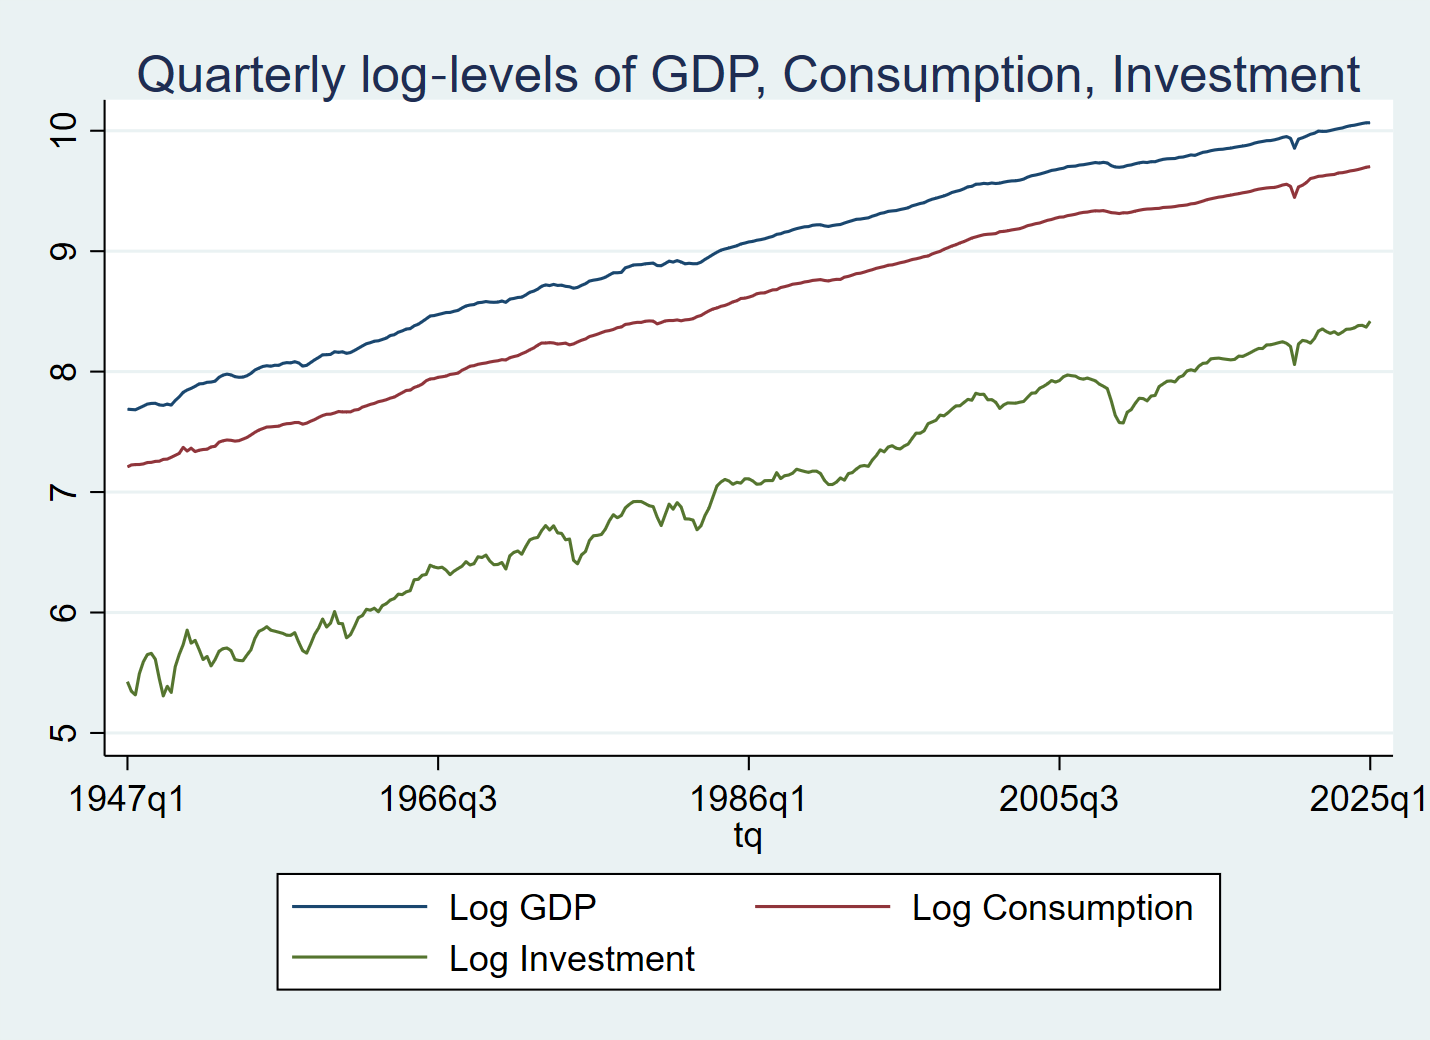
\includegraphics[width=0.8\textwidth]{a.png}
    \end{figure}
\end{autosolution}

\begin{autosolution}
    \

    % The OLS estimators are
    % \begin{align}
    %     \hat\beta_2
    %     &= \frac{\sum_{t}(t-\bar t)\,(y_t-\bar y)}{\sum_{t}(t-\bar t)^2}, 
    %     \quad
    %     \hat\beta_1 = \bar y - \hat\beta_2\,\bar t,
    % \end{align}
    % where
    % $\bar t = \frac1N\sum_t t$, $\bar y = \frac1N\sum_t y_t$, $N$ is the number of quarters, $y_t$ is the log of three variables.
    Let $\mathbf{X}=(\mathbf{1},\,\mathbf{t})$ be the $N\times2$ design matrix, with rows $(1,t)$, and $\mathbf{y}=(y_1,\dots,y_N)'$.  Then the OLS estimator is
    \[
    \begin{pmatrix}\hat\beta_1\\[0.2em]\hat\beta_2\end{pmatrix}
    = (\mathbf{X}'\mathbf{X})^{-1}\mathbf{X}'\mathbf{y}
    =\frac{1}{S_{tt}}
    \begin{pmatrix}
    \sum_t t^2 & -\sum_t t \\[0.4em]
    -\sum_t t & \sum_t 1
    \end{pmatrix}
    \begin{pmatrix}
    \sum_t y_t \\[0.2em]
    \sum_t t\,y_t
    \end{pmatrix},
    \]
    where
    \[
    \bar t = \frac1N\sum_{t=1}^N t,\quad
    \bar y = \frac1N\sum_{t=1}^N y_t,\quad
    S_{tt} = \sum_{t=1}^N(t-\bar t)^2.
    \]
    Equivalently,
    \[
    \hat\beta_2
    = \frac{\sum_{t=1}^N (t-\bar t)(\,y_t-\bar y)}{\sum_{t=1}^N (t-\bar t)^2},
    \quad
    \hat\beta_1 = \bar y - \hat\beta_2\,\bar t.
    \]
    The fitted values and residuals are
    \[
    \hat y_t = \hat\beta_1 + \hat\beta_2\,t,\qquad
    \hat u_t = y_t - \hat y_t.
    \]
    $y_t$ is the log of three variables: GDP, PCE, and GPDI.
    The estimated models are as below:
    \begin{table}[h!]
    \centering
        \begin{tabular}{lcccc}
        \toprule
        Window & Series & $\hat\beta_1$ & $\hat\beta_2$ (per qtr) & Annualized Growth (\%) \\
        \midrule
        1965\,Q1--2006\,Q4 & $\ln\mathrm{GDP}$  & $7.8509$  & $0.0077707$ & $3.11$ \\
                        & $\ln\mathrm{PCE}$  & $7.3017$  & $0.0083520$ & $3.34$ \\
                        & $\ln\mathrm{GPDI}$ & $5.4989$  & $0.0100216$ & $4.01$ \\[6pt]
        2007\,Q1--2019\,Q4 & $\ln\mathrm{GDP}$  & $8.4997$  & $0.0048888$ & $1.96$ \\
                        & $\ln\mathrm{PCE}$  & $8.0947$  & $0.0049259$ & $1.97$ \\
                        & $\ln\mathrm{GPDI}$ & $5.2006$  & $0.0104206$ & $4.17$ \\[6pt]
        2007\,Q1--2022\,Q2 & $\ln\mathrm{GDP}$  & $8.4867$  & $0.0049376$ & $1.98$ \\
                        & $\ln\mathrm{PCE}$  & $8.0394$  & $0.0051370$ & $2.05$ \\
                        & $\ln\mathrm{GPDI}$ & $5.3432$  & $0.0098678$ & $3.95$ \\
        \bottomrule
        \end{tabular}
        \caption{Trend regression estimates and annualized growth rates}
    \end{table}


\end{autosolution}

\begin{autosolution}    
    \

    $\hat\beta_2$ measures the \emph{average quarterly} change in $\ln y_t$.  

    The \emph{approximate quarterly growth rate} is $\hat\beta_2\times100\%$. 

    The \emph{exact annualized growth rate} is 
    \[
    \bigl(e^{4\,\hat\beta_2}-1\bigr)\times100\% \approx 4 \hat\beta_2 \times 100\%,
    \]
    \begin{itemize}
        \item \textbf{1965--2006:}  
        GDP grows at about $0.78\%$ per quarter $\Rightarrow$ $3.11\%$ per year;  
        Consumption: $0.84\%$ qtr $\Rightarrow$ $3.34\%$ yr;  
        Investment: $1.00\%$ qtr $\Rightarrow$ $4.01\%$ yr.  

        \item \textbf{2007--2019:}  
        GDP/Consumption trend roughly halves to ≈$0.49\%$ qtr $\Rightarrow$ ≈$1.96\%$ yr.  
        Investment trend remains high, ≈$1.04\%$ qtr $\Rightarrow$ $4.17\%$ yr.

        \item \textbf{2007--2022:}  
        GDP/Consumption trend stays near $2.05\%$ annualized; Investment trend slightly eases to $3.95\%$.

        % \item \textbf{$R^2$ values (not shown)} confirm near‐perfect fit in the long sample ($R^2>0.99$),  
        % while in the shorter windows investment’s $R^2$ falls (to ~0.72), reflecting larger cyclical deviations from the linear trend.
    \end{itemize}
    GDP and PCE grow at a similar rate, but investment grow faster, at about twice the rate of GDP and PCE.
\end{autosolution}

\begin{autosolution}
    \

    The ($k$th) sample autocorrelation of $\{\hat u_t\}$ is
    \[
    \hat\rho(k)
    = \frac{\displaystyle\sum_{t=k+1}^N \hat u_t\,\hat u_{t-k}}
        {\displaystyle\sum_{t=1}^N \hat u_t^2},
    \qquad k=0,1,2,\dots.
    \]
    We compute $\hat\rho(k)$ for $k=1,\dots,K$ (here $K=8$) in each subsample to assess the persistence of residual cycles.

\end{autosolution}


\begin{autosolution}
    \

    \begin{figure}[ht]
        \centering
        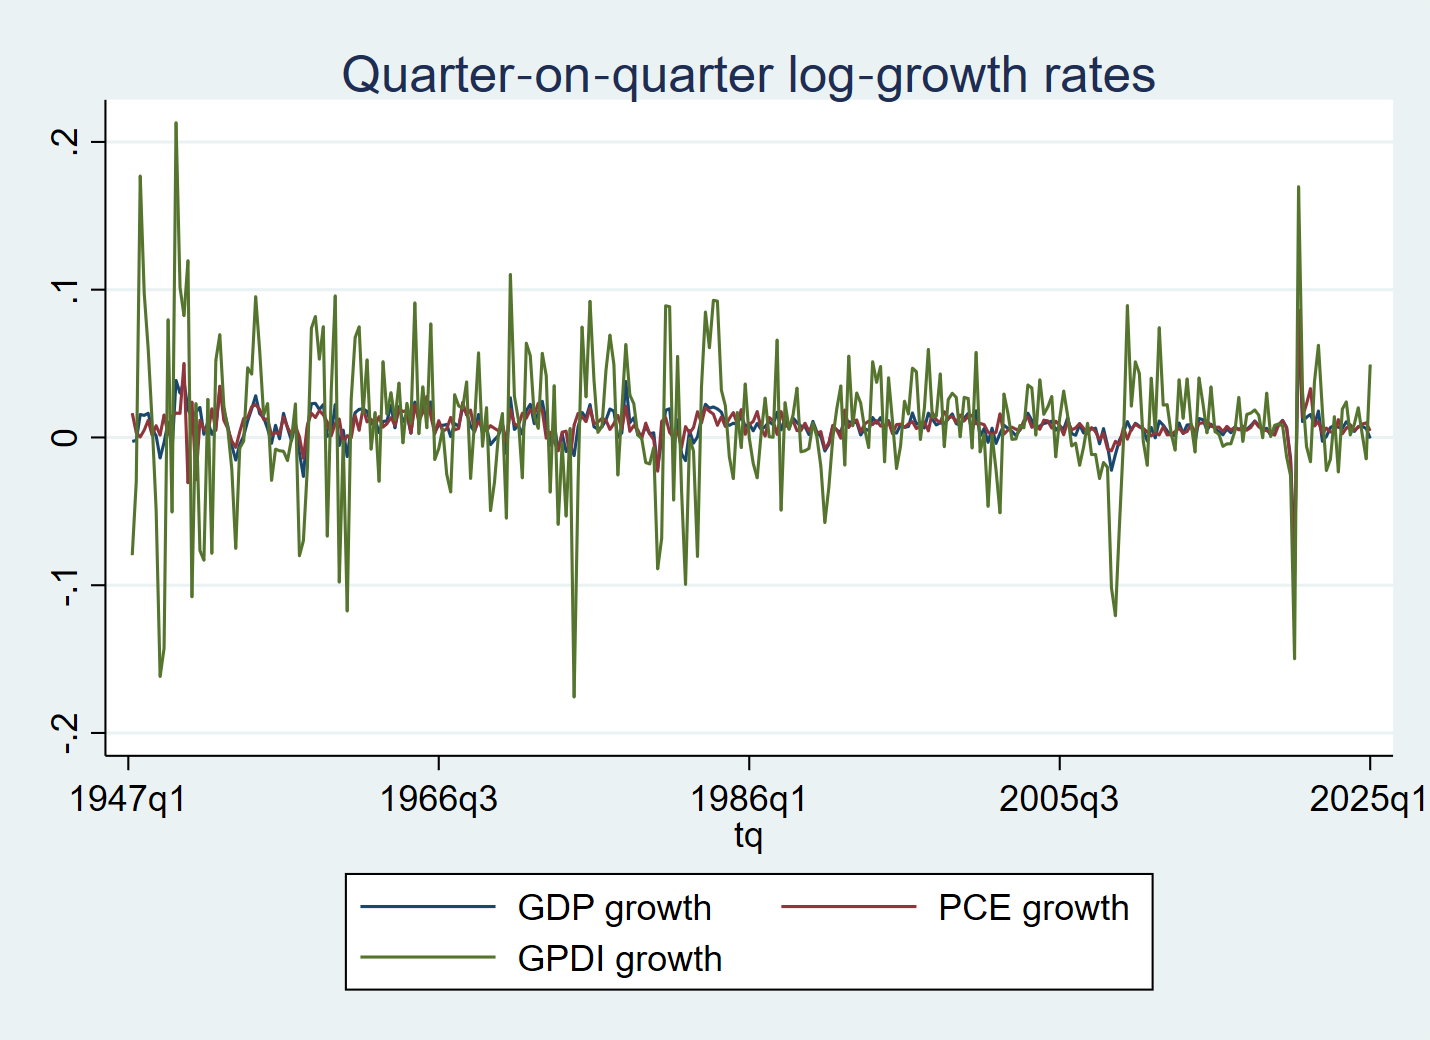
\includegraphics[width=0.8\textwidth]{e.png}
    \end{figure}    
\end{autosolution}


\begin{autosolution}
    \

    For each series $g_t\in\{\Delta y_t,\Delta c_t,\Delta i_t\}$ in a given subsample of length $M$, we compute
    \[
    \bar g = \frac{1}{M}\sum_{t=1}^M g_t,
    \qquad
    s_g = \sqrt{\frac{1}{M-1}\sum_{t=1}^M\bigl(g_t-\bar g\bigr)^2}.
    \]
    These compare the \emph{average realized growth} $\bar g$ with the \emph{trend-based} quarterly slope $\hat\beta_2$, and measure cyclical volatility via $s_g$.
    \begin{table}[ht]
        \centering
        \begin{tabular}{llrrrrr}
        \toprule
        Window & Series & Obs & Mean of $\Delta\ln y$ & Std. of $\Delta\ln y$ & $\hat\beta_2$ (per qtr) \\
        \midrule
        1965\,Q2--2006\,Q4
        & GDP    & 167 & 0.0079889 & 0.0082641 & 0.0077707 \\
        & PCE    & 167 & 0.0086664 & 0.0067471 & 0.0083520 \\
        & GPDI   & 167 & 0.0100079 & 0.0391054 & 0.0100216 \\
        \addlinespace
        2007\,Q2--2019\,Q4
        & GDP    &  51 & 0.0045828 & 0.0061137 & 0.0048888 \\
        & PCE    &  51 & 0.0045793 & 0.0043225 & 0.0049259 \\
        & GPDI   &  51 & 0.0058344 & 0.0346509 & 0.0104206 \\
        \addlinespace
        2007\,Q2--2022\,Q2
        & GDP    &  61 & 0.0045452 & 0.0159656 & 0.0049376 \\
        & PCE    &  61 & 0.0050521 & 0.0175900 & 0.0051370 \\
        & GPDI   &  61 & 0.0064772 & 0.0444316 & 0.0098678 \\
        \bottomrule
        \end{tabular}
    \end{table}

    \textbf{Comparison to part (b):}
    \begin{itemize}
        \item \emph{1965 Q2-2006 Q4:} The sample means of $\Delta\ln y$ for GDP (0.00799), PCE (0.00867) and GPDI (0.01001) are almost identical to the estimated quarterly trend slopes $\hat\beta_2$ (0.0077707, 0.0083520, 0.0100216). 
        This confirms that, over the long sample, the linear-trend regression accurately captures the average growth rate.
        \item \emph{2007 Q2-2019 Q4:} GDP and PCE mean growth rates ($\approx$0.00458) lie slightly below their $\hat\beta_2$ ($\approx$0.00489 and 0.00493), reflecting that downturns (2008-09 crisis) pull the sample average below the fitted trend. 
        For GPDI, the mean (0.00583) is markedly below its trend slope (0.01042), since investment experienced large negative shocks that the OLS trend, minimizing squared errors, spreads more evenly across the sample.
        \item \emph{2007 Q2-2022 Q2:} Including the COVID-19 shock further widens the gap: GDP and PCE means (0.00455, 0.00505) remain below their slopes (0.00494, 0.00514), and investment's mean (0.00648) stays well under its slope (0.00987). 
        This again shows that severe cyclical downturns pull down the simple average growth below the fitted linear trend.
    \end{itemize}
\end{autosolution}

\begin{autosolution}
    \

    \begin{table}[ht]
        \centering
        \begin{tabular}{llrr}
        \toprule
        Window               & Series & Mean of $\Delta\ln y$ & Std.\ dev.\ of $\Delta\ln y$ \\
        \midrule
        1965\,Q2--1983\,Q4   & GDP    & 0.0078863              & 0.0109888                    \\
                             & PCE    & 0.0086857              & 0.0085560                    \\
                             & GPDI   & 0.0091587              & 0.0504674                    \\
        \addlinespace
        1984\,Q1--2006\,Q4   & GDP    & 0.0080725              & 0.0051354                    \\
                             & PCE    & 0.0086507              & 0.0048490                    \\
                             & GPDI   & 0.0107001              & 0.0267834                    \\
        \bottomrule
        \end{tabular}
    \end{table}

    \begin{itemize}
        \item \emph{Mean growth rates:}  
            GDP’s average growth rises slightly from 0.7886\% to 0.8073\%;  
            PCE falls marginally from 0.8686\% to 0.8651\%;  
            GPDI increases from 0.9159\% to 1.0700\%.  
            Overall, the mean growth rates remain essentially unchanged in magnitude.
        \item \emph{Volatility:}  
            All three series exhibit a dramatic reduction in standard deviation.  
            \begin{itemize}
                \item GDP's $\sigma$ falls from 1.10\% to 0.51\%.  
                \item PCE's $\sigma$ falls from 0.86\% to 0.48\%.  
                \item GPDI's $\sigma$ falls from 5.05\% to 2.68\%.  
            \end{itemize}
        This confirms the \emph{Great Moderation}—after 1984, while average growth remained stable, business-cycle volatility was substantially dampened.
    \end{itemize}  
\end{autosolution}



\section{Problem 2}

\begin{autosolution}
    \

    \subsection*{Weak Stationarity}

    A process $\{y_t\}$ is weakly stationary if
    \[
    \mathbb{E}[y_t]=\mu\quad \forall t,
    \quad 
    \operatorname{Cov}(y_t,y_{t-k})=\gamma_k \text{ depends only on }k.
    \]
    Here
    \[
    \mathbb{E}[y_t]
    =\sum_{j=0}^3\psi_j\,\mathbb{E}[u_{t-j}]
    =0,
    \]
    so the mean is constant.  Next,
    \[
    \operatorname{Cov}(y_t,y_{t-k})
    =\mathbb{E}\bigl[y_t\,y_{t-k}\bigr]
    =\sum_{j=0}^3\sum_{i=0}^3\psi_j\psi_i\,
    \mathbb{E}\bigl[u_{t-j}u_{t-k-i}\bigr].
    \]
    Since $\mathbb{E}[u_su_r]=0$ for $s\neq r$, only terms with
    $t-j = t-k-i$ survive, so $\operatorname{Cov}(y_t,y_{t-k})$ depends on $k$ alone.  
    Hence $\{y_t\}$ is weakly stationary.

    \subsection*{Strict Stationarity}

    If $\{u_t\}$ is strictly stationary (e.g.\ i.i.d.), then any finite-order linear filter
    $\sum_{j=0}^3\psi_j\,u_{t-j}$
    yields a strictly stationary $\{y_t\}$.  Thus under i.i.d.\ innovations, $y_t$ is strictly stationary.
\end{autosolution}

\begin{autosolution}
    \

    Define $\gamma_k = \operatorname{Cov}(y_t,y_{t-k})$.  With $\psi_j$ as above,
    \[
    \gamma_k
    =\sum_{j=0}^3\sum_{i=0}^3\psi_j\psi_i\,
    E[u_{t-j}u_{t-k-i}]
    =\sum_{j=0}^3 \psi_j\,\psi_{j-k},
    \]
    interpreting $\psi_{m}=0$ for $m<0$ or $m>3$.

    Thus:
    \begin{align*}
    \gamma_0
    &=\sum_{j=0}^3\psi_j^2
    =1^2 + (-2.4)^2 + 0.8^2 + (-0.4)^2
    =7.56,\\
    \gamma_1
    &=\psi_0\psi_1 + \psi_1\psi_2 + \psi_2\psi_3
    =1\cdot(-2.4) + (-2.4)\cdot0.8 + 0.8\cdot(-0.4)
    =-4.64,\\
    \gamma_2
    &=\psi_0\psi_2 + \psi_1\psi_3
    =1\cdot0.8 + (-2.4)\cdot(-0.4)
    =1.76,\\
    \gamma_3
    &=\psi_0\psi_3
    =1\cdot(-0.4)
    =-0.4,\\
    \gamma_k&=0\quad\text{for }|k|\ge4.
    \end{align*}
    The autocorrelation is $\rho_k=\gamma_k/\gamma_0$.
\end{autosolution}


\begin{autosolution}
    \

    Consider
    \[
    S_T = \sum_{t=1}^T y_t,
    \qquad
    V_T = \mathbb{V}[S_T]
    =\sum_{i=1}^T\sum_{j=1}^T\gamma_{i-j}.
    \]
    Re-index $h=j-i$:
    \[
    V_T = \sum_{h=-(T-1)}^{T-1} (T-|h|)\,\gamma_h.
    \]
    Hence
    \[
    \mathbb{V}\left[\tfrac1{\sqrt T}S_T\right]
    =\frac{V_T}{T}
    =\gamma_0 + 2\sum_{h=1}^{T-1}\Bigl(1-\tfrac{h}{T}\Bigr)\gamma_h.
    \]
    As $T\to\infty$, $\frac{h}{T}\to0$ for fixed $h$, and $\gamma_h=0$ for $h\ge4$, so
    \[
    \lim_{T\to\infty}
    \mathbb{V}\left[\tfrac1{\sqrt T}S_T\right]
    =\gamma_0 + 2(\gamma_1+\gamma_2+\gamma_3)
    =7.56 + 2(-4.64 + 1.76 - 0.4)
    =1.
    \]
\end{autosolution}

\begin{autosolution}
    \

    Assume $\{u_t\}$ is i.i.d.\ with $\mathbb{E}[u_t]=0$, $\mathbb{V}[u_t]=\sigma^2$.
    \subsection*{Strict Stationarity}

    $x_t=f(u_t,u_{t-4})$ depends on two i.i.d.\ draws; hence its joint distributions do not change with shifts in $t$.  So $\{x_t\}$ is strictly stationary.

    \subsection*{Ergodicity}

    An i.i.d.\ sequence is ergodic and any measurable function of it remains ergodic.  Thus $\{x_t\}$ is ergodic.

    \subsection*{White-Noise Properties}
    \begin{itemize}
    \item $\mathbb{E}[x_t] = \mathbb{E}[u_t]\mathbb{E}[u_{t-4}] = 0.$
    \item For $k\neq0$,
    \[
        \operatorname{Cov}(x_t,x_{t-k})
        =\mathbb{E}[u_t u_{t-4} u_{t-k} u_{t-k-4}]
        =0,
    \]
    since among the four factors at least one is independent with zero mean.
    \end{itemize}
    Hence $\{x_t\}$ is zero-mean uncorrelated white noise, but not i.i.d.\ (since $x_t$ and $x_{t+4}$ share $u_t$).
\end{autosolution}

\begin{autosolution}
    \

    We have:
    \[
    \mathbb{E}\left[\tfrac1T \sum_{t=1}^T x_t\right]
    =\tfrac1T\sum_{t=1}^T \mathbb{E}[x_t]
    =0,
    \]
    and since $\operatorname{Cov}(x_i,x_j)=0$ for $i\neq j$,
    \[
    \mathbb{V}\left[\tfrac1{\sqrt T}\sum_{t=1}^T x_t\right]
    =\frac{1}{T}\sum_{t=1}^T \mathbb{V}[x_t]
    =\sigma^4.
    \]
\end{autosolution}

\end{document}

